\documentclass[11pt]{article}
\usepackage{apacite}
\usepackage{graphicx}
\graphicspath{ {./images/} }
\begin{document}
\section{Case Study}
\subsection{Prototype}
We would like to show the features of our product and with some users evaluate our product and get feedback from the users for future improvement.
Based on the model of House and Hill 1997 ~\cite{houdeChapter16What1997}, we develop both "Role" and "Look and feel" prototype to test the research question of our concern. We intend to provide both full overview of the functionality and concrete experience successively via each prototype.
In the "Role" prototype, we use "Role Playing". We also shoot a video depicting how our mirror functions. Regarding "Look and feel" prototype, we build a mirror surface, user can draw on it using the finger movement.
\begin{figure}[h]
\caption{The components of MagicMirror}
\centering
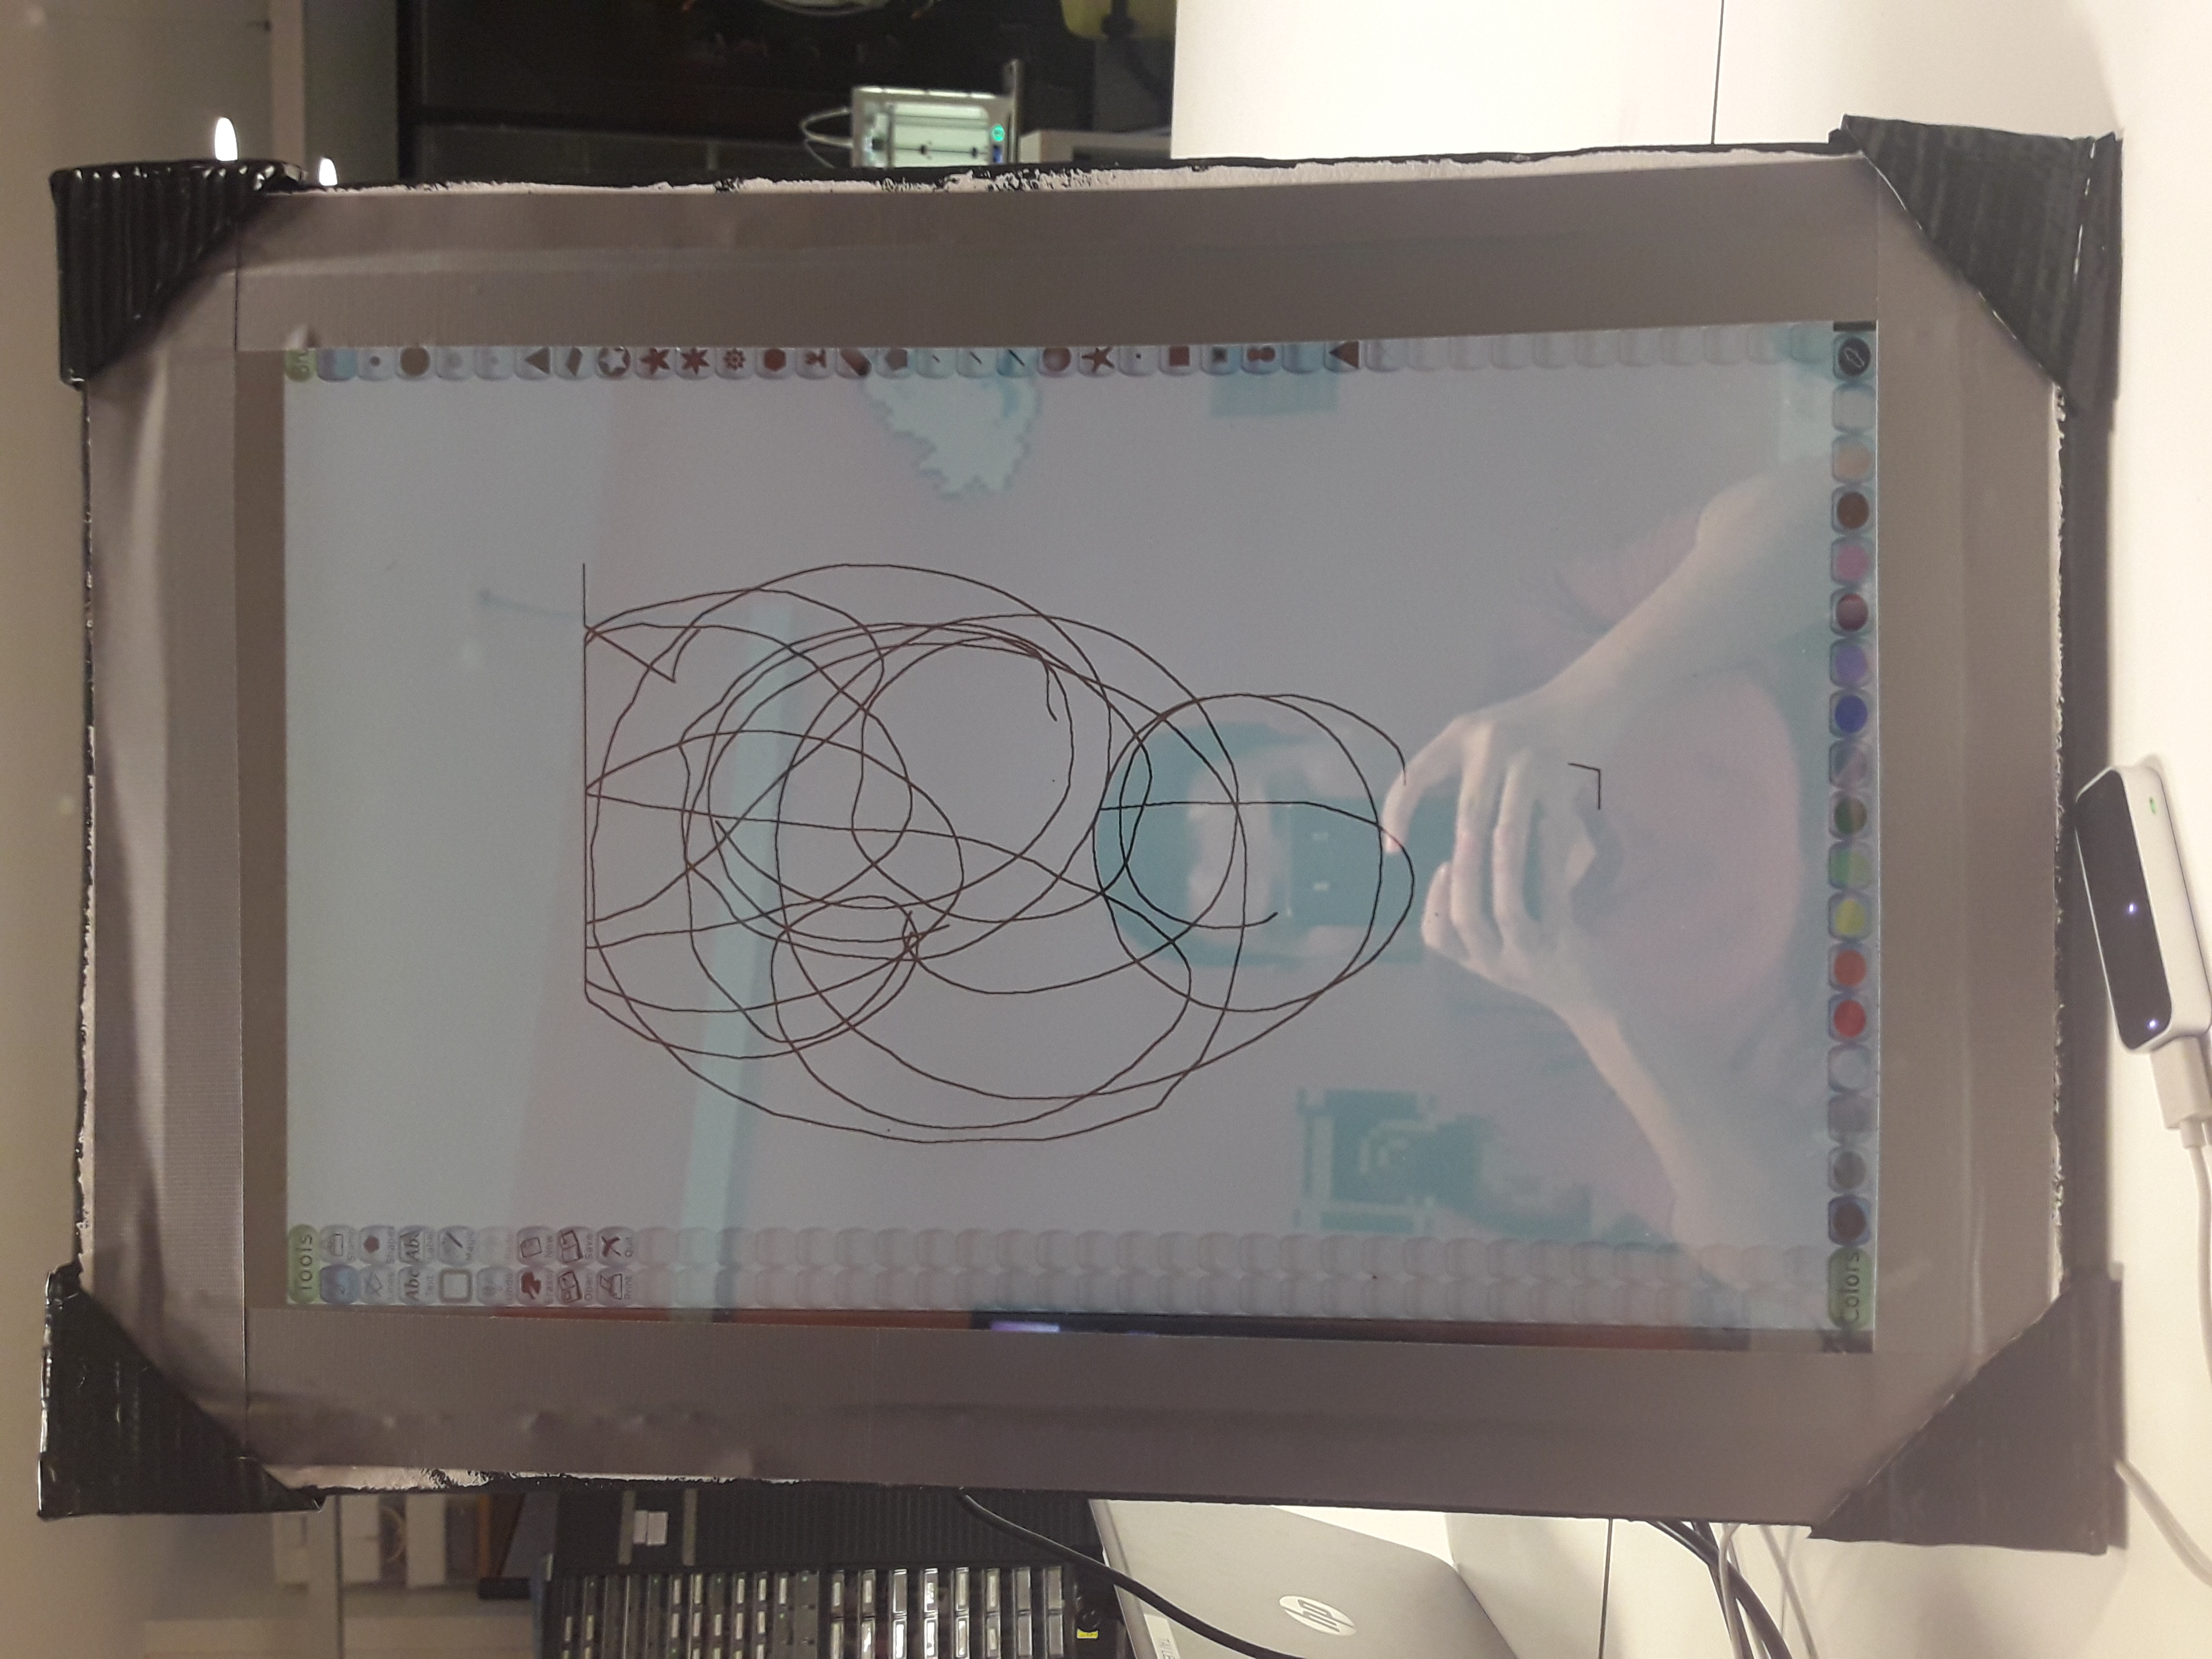
\includegraphics[width=10cm, height=7cm, angle=-90]{prototype}
\end{figure}
\linebreak
\textit{Hardware}
A glass with reflection solar film (80\% reflection surface), a Leap Motion, a 24" LCD.
\textit{Software}
Touchless for Windows an Leap Motion application developed by Leap Motion Gallery, Tux Paint.
\bibliographystyle{apacite}
\bibliography{ref}

\end{document}
